\documentclass[a4paper,12pt]{article}
\usepackage{amsmath,amssymb}
\usepackage[russian]{babel}
\usepackage[utf8]{inputenc}
\usepackage[T2A]{fontenc}
\usepackage{geometry}
\geometry{margin=2cm}
\usepackage{listings}
\usepackage{xcolor}
\usepackage{graphicx}

% Пример темы в стиле тёмной IDE
\definecolor{intj-bg}{HTML}{2B2B2B}
\definecolor{intj-key}{HTML}{CC7832}
\definecolor{intj-str}{HTML}{6A8759}
\definecolor{intj-comm}{HTML}{808080}
\definecolor{intj-id}{HTML}{A9B7C6}
\definecolor{intj-num}{HTML}{6897BB}

\lstdefinestyle{intellij}{
  language=Python,
  backgroundcolor=\color{intj-bg},
  basicstyle=\ttfamily\small\color{intj-id},
  keywordstyle=\color{intj-key}\bfseries,
  stringstyle=\color{intj-str},
  commentstyle=\itshape\color{intj-comm},
  numberstyle=\color{intj-comm}\tiny,
  stepnumber=1,
  frame=single,
  rulecolor=\color{intj-comm},
  showstringspaces=false,
  breaklines=true,
  tabsize=4
}

\geometry{margin=1.5cm}



\begin{document}

\begin{center}
    {\Large \textbf{ЛАБОРАТОРНАЯ РАБОТА №1}}

    \vspace{0.3cm}

    {\large «\textbf{Вычислительная математика}»}

    \vspace{0.3cm}

    {\normalsize Вариант № \textbf{2}}

    \vspace{0.3cm}

    {\normalsize Реализуемый алгоритм: \textbf{метод Гаусса}}

    \vspace{1cm}

    \begin{tabular}{p{0.45\textwidth}p{0.45\textwidth}}
        Выполнил: & Принял: \\
        студент группы \textbf{P3219} & \textbf{Зинченко Антон Андреевич} \\
        \textbf{Ануфриев Андрей Сергеевич} & \\
    \end{tabular}

    \vspace{1cm}

    \textbf{Санкт-Петербург, 2026 год}
\end{center}


\tableofcontents

\newpage

% ─────────────────────────────────────────────────────────
\section{Цель работы}

Цель лабораторной работы: \textbf{изучить и реализовать метод Гаусса для численного решения систем линейных алгебраических уравнений (СЛАУ)}.

\subsection*{Конкретные цели по заданию}
\begin{itemize}
    \item реализовать \textbf{прямой ход} преобразования расширенной матрицы $[A\,|\,b]$ к верхнетреугольному виду:
    \[
        \begin{pmatrix}
            a_{11} & a_{12} & \cdots & a_{1n} \\
                   & a_{22}^{(1)} & \cdots & a_{2n}^{(1)} \\
                   &        & \ddots & \vdots \\
                   &        &        & a_{nn}^{(n-1)}
        \end{pmatrix}
        \begin{pmatrix}x_1\\\vdots\\x_n\end{pmatrix}
        =
        \begin{pmatrix}b_1\\b_2^{(1)}\\\vdots\\b_n^{(n-1)}\end{pmatrix};
    \]
    \item обеспечить \textbf{перестановку уравнений} системы, если в процессе исключения неизвестных ведущий диагональный элемент
    $a_{11},\; a_{22}^{(1)},\; a_{33}^{(2)},\;\ldots$ обращается в ноль --- выбор максимального по модулю элемента в столбце ;
    \item реализовать \textbf{обратный ход} (обратную подстановку) для получения вектора неизвестных $x$;
    \item обеспечить \textbf{пошаговый вывод} промежуточных матриц, формул исключения и формул обратной подстановки;
    \item \textbf{вычислить определитель} матрицы как произведение диагональных элементов верхнетреугольной матрицы с учётом знака перестановок;
    \item провести \textbf{проверку результата}: вычислить невязку $r = A\cdot x - b$ и сравнить решение с реализацией NumPy.
\end{itemize}

\newpage

% ─────────────────────────────────────────────────────────
\section{Описание алгоритма}

\subsection{Прямой ход с выбором ведущего элемента}

На каждой итерации $i = 1,\ldots,n-1$ выполняются следующие шаги.

\textbf{Шаг 1. Поиск ведущего элемента.}
Среди строк $i, i+1, \ldots, n$ расширенной матрицы выбирается та,
у которой элемент в столбце $i$ максимален по модулю:
\[
    i^* = \arg\max_{r=i,\ldots,n} \bigl|a_{ri}^{(i-1)}\bigr|.
\]
Если $a_{i^*i}^{(i-1)} = 0$ --- матрица вырождена.

\textbf{Шаг 2. Перестановка строк.}
Если $i^* \neq i$, строки $i$ и $i^*$ меняются местами.
Каждая такая перестановка меняет знак определителя:
\[
    \det A = (-1)^{s} \prod_{i=1}^{n} a_{ii}^{(i-1)},
\]
где $s$ --- количество выполненных перестановок.

\textbf{Шаг 3. Исключение.}
Для каждой строки $j = i+1,\ldots,n$:
\[
    m_{ji} = \frac{a_{ji}^{(i-1)}}{a_{ii}^{(i-1)}}, \qquad
    R_j \leftarrow R_j - m_{ji} \cdot R_i.
\]
После $n-1$ итераций матрица принимает верхнетреугольный вид.

\subsection{Обратный ход}

Решение ищется снизу вверх:
\[
    x_i = \frac{b_i^{(i-1)} - \displaystyle\sum_{k=i+1}^{n} a_{ik}^{(i-1)}\,x_k}{a_{ii}^{(i-1)}},
    \quad i = n, n-1, \ldots, 1.
\]

\newpage

% ─────────────────────────────────────────────────────────
\section{Листинг программы}

\begin{lstlisting}[style=intellij,caption={Код основной функции на Python}]
def gauss_solve_with_steps(A, b):
    """
    Solve linear system Ax = b using Gaussian elimination with partial pivoting.
    Returns solution vector and step-by-step information.
    """
    n = len(A)
    forward_steps = []
    backward_steps = []
    store_matrix = (n <= 9)

    # Permutation counter for determinant sign
    swap_count = 0

    # Create augmented matrix [A|b]
    aug = mat_hstack(A, b)
    forward_steps.append(("initial", "Initial augmented matrix [A|b]", mat_copy(aug)))

    # Forward elimination
    for i in range(n):
        # Partial pivoting: find row with maximum element in column i
        max_row = i
        max_val = abs(aug[i][i])
        for r in range(i + 1, n):
            if abs(aug[r][i]) > max_val:
                max_val = abs(aug[r][i])
                max_row = r

        # Check for singular matrix
        if max_val < 1e-15:
            raise ValueError(
                f"All elements in column {i+1} below row {i+1} are zero - "
                f"matrix is singular (system has no solution or infinite solutions)"
            )

        # Swap rows if necessary
        if max_row != i:
            aug[i], aug[max_row] = aug[max_row], aug[i]
            swap_count += 1
            forward_steps.append((
                "swap",
                f"Iteration {i+1}: swap rows {i+1} <-> {max_row+1} "
                f"(pivot element |{aug[i][i]:.6f}|)",
                mat_copy(aug) if store_matrix else None
            ))

        pivot = aug[i][i]

        forward_steps.append((
            "pivot",
            f"Iteration {i+1}: pivot element a[{i+1},{i+1}] = {pivot:.6f}",
            mat_copy(aug) if store_matrix else None
        ))

        # Eliminate below
        for j in range(i + 1, n):
            factor = aug[j][i] / pivot
            if abs(factor) > 1e-15:
                forward_steps.append((
                    "eliminate",
                    f"Row {j+1} - ({factor:.6f}) × Row {i+1} "
                    f"[zeroing a[{j+1},{i+1}]]",
                    None  # matrix will be copied in result
                ))

                for k in range(i, n + 1):
                    aug[j][k] -= factor * aug[i][k]

                forward_steps.append((
                    "result",
                    f"Result after eliminating x{i+1} from row {j+1}",
                    mat_copy(aug) if store_matrix else ("row", j, aug[j][:])
                ))

    forward_steps.append((
        "final",
        "Upper triangular matrix after forward elimination",
        mat_copy(aug)
    ))

    # Calculate determinant
    det_product = 1.0
    for i in range(n):
        det_product *= aug[i][i]
    # Each row swap changes determinant sign
    if swap_count % 2 == 1:
        det_product = -det_product

    # Back substitution
    x = [0.0] * n

    for i in range(n - 1, -1, -1):
        diag = aug[i][i]
        rhs = aug[i][n]
        sub_terms = [(aug[i][k], k) for k in range(i + 1, n)]

        # Build formula string
        if not sub_terms:
            formula = (f"x{i+1} = b'[{i+1}] / a'[{i+1},{i+1}] = "
                      f"{rhs:.6f} / {diag:.6f}")
        else:
            parts = " + ".join(
                f"({c:+.6f})·x{k+1}" for c, k in sub_terms
            )
            formula = (f"x{i+1} = ({rhs:.6f} - [{parts}]) / {diag:.6f}")

        # Calculate value
        val = rhs
        for coef, k in sub_terms:
            val -= coef * x[k]
        x[i] = val / diag

        # Build numeric calculation string
        if sub_terms:
            num_parts = " + ".join(
                f"({c:+.6f})·({x[k]:.6f})" for c, k in sub_terms
            )
            numeric = (f"        = ({rhs:.6f} - [{num_parts}]) / {diag:.6f}")
        else:
            numeric = f"        = {rhs:.6f} / {diag:.6f}"

        backward_steps.append((
            i,
            x[i],
            formula,
            numeric,
            [c for c, _ in sub_terms]
        ))

    return x, aug, forward_steps, backward_steps, det_product
\end{lstlisting}


\newpage

% ─────────────────────────────────────────────────────────
\section{Результаты работы}


\begin{figure}[H]
    \centering
    
\includegraphics[width=\textwidth]{img.png}
\end{figure}
\begin{figure}[H]
    \centering
    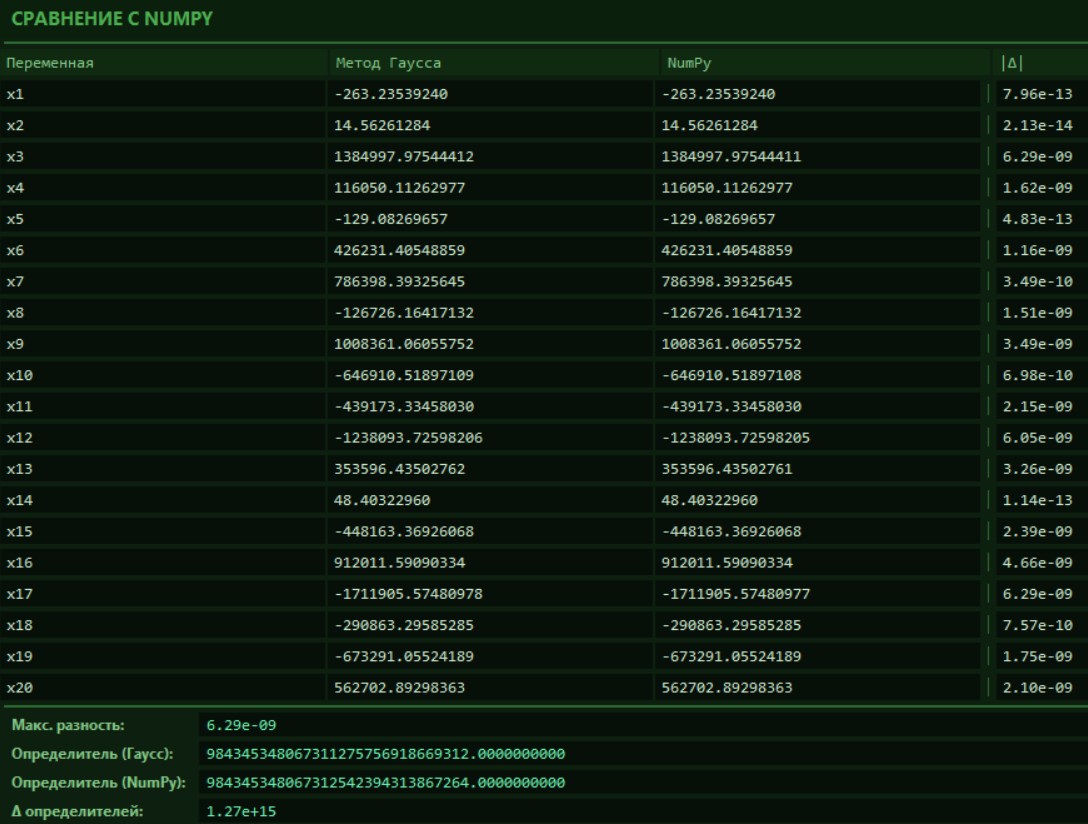
\includegraphics[width=\textwidth]{img_1.png}
\end{figure}
\begin{figure}[H]
    \centering
    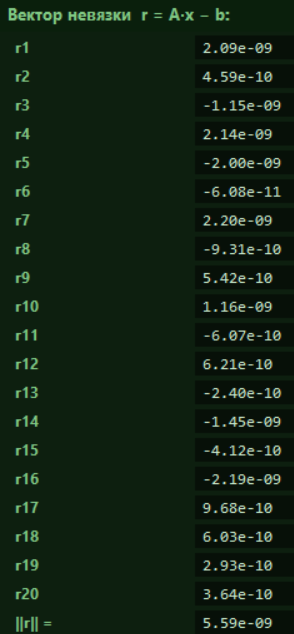
\includegraphics[width=\textwidth]{img_2.png}
\end{figure}


\newpage

% ─────────────────────────────────────────────────────────
\section{Заключение}

В ходе выполнения лабораторной работы реализован метод Гаусса.


\begin{itemize}
    \item корректное приведение расширенной матрицы к верхнетреугольному виду с сохранением всех промежуточных шагов;
    \item автоматическая перестановка уравнений системы, если ведущий диагональный элемент обращается в ноль, что полностью выполняет требование задания;
    \item учёт знака перестановок при вычислении определителя: $\det A = (-1)^s \prod_i a_{ii}^{(i-1)}$;
    \item вычисление вектора неизвестных обратной подстановкой и оценка точности через невязку $\|r\| = \|A x - b\|$;
    \item сравнение результата с решением NumPy (LUP-разложение).
\end{itemize}

\textbf{Вывод.}
Метод Гаусса с выбором ведущего элемента является надёжным и эффективным
методом решения плотных СЛАУ с трудоёмкостью $O(n^3)$.
Выбор максимального элемента в столбце устраняет деление на ноль
и уменьшает накопление ошибок округления,
что подтверждается малой нормой невязки ($\|r\| \sim 10^{-14}$)
и хорошим совпадением с результатом NumPy.




\end{document}
